%/////////////////////////////////////////////////
%/
\chapter{Implementation}
%/
%/////////////////////////////////////////////////
\label{chap:implementation}

%/////////////////////////////////////////////////
%/
\section{SMT-RAT}
%/
%/////////////////////////////////////////////////
\label{sec:smt-rat}
We implement our work in the SMT toolbox called SMT-RAT which is entirely written in C++.
Modules are the elementary architectural component of SMT-RAT.
SMT-RAT is very extensible because of the modules.
It is possible to integrate SMT-RAT with new modules which can be act as a theory solver.
The execution order of modules are defined in a strategy which is a directed graph.
Depending on the requirement, different strategies may contain different module references in different order.
Modules can have settings arguments.
So, several strategies can have same order of modules but with different settings parameter.
Settings are some configurations which can be used to configure a module in different ways without changing the code.
SMT-RAT takes a formula as an input.
We also have to set the name of the strategy to inform SMT-RAT that which modules are needs to execute in which order.
Depending on the implementations of the modules, SMT-RAT decides satisfiability of the input formula.
SMT-RAT outputs SAT if a formula satisfies, UNSAT if a formula unsatisfies and UNKNOWN if the result is not decidable.
The Figure \ref{fig:overview_architecture_SMT-RAT} shows an overview architecture of SMT-RAT.\newline

\noindent We can see the toolbox has various kinds of modules for example, \textit{SATModule}, \textit{LRAModule}, \textit{NRAILModule} and so on.
Here \textit{SATModule} is a SAT solver and there are other modules which are theory solvers e.g. \textit{LRAModule}, \textit{NRAModule}.
Besides SAT solver and theory solvers, there are other modules which are only responsible for some prepossessing, e.g.,\textit{FPPModule}.
The module \textit{NRAILModule} is our implemented module.
We also can see there are different strategies available and one of them is \textit{NRARefinmentSolver} which is our defined strategy.
In strategies, the modules are connected hierarchically as a directed graph.
A module in a strategy can only use its direct successor module for computation because a module may need help of another module.
A module is addressed as backend and frontend for its direct ancestor and successor module, respectively.
Note that, a module can never know which module is its successor or ancestor module.\newline

\begin{figure}[ht!]
  \centering
  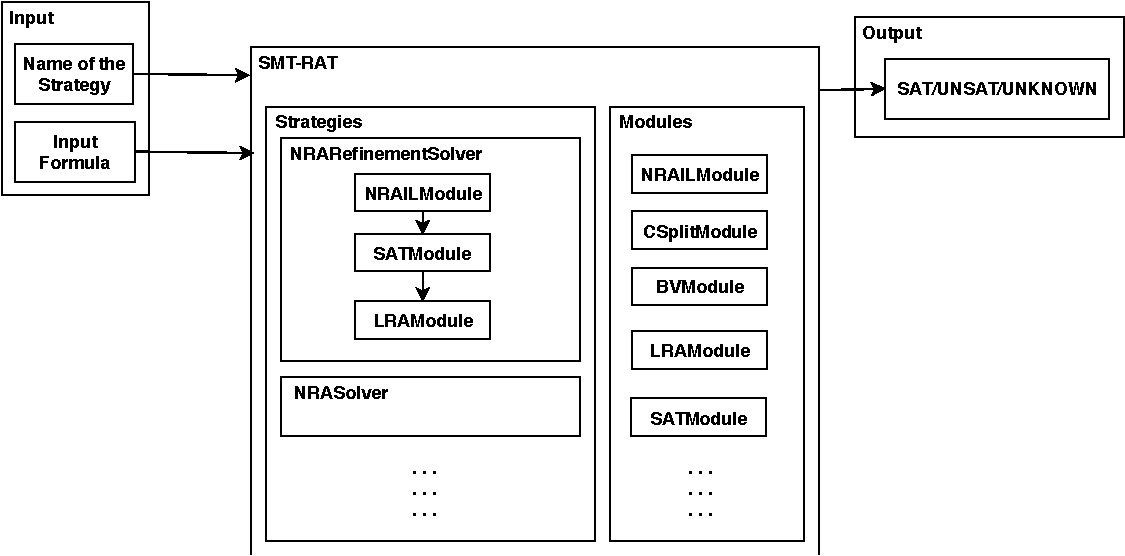
\includegraphics[width=.9\linewidth]{./figures/smtrat-arch.pdf}
  \caption{Overview architecture of SMT-RAT}
  \label{fig:overview_architecture_SMT-RAT}
\end{figure}


%/////////////////////////////////////////////////
%/
\section{NRARefinmentSolver}
%/
%/////////////////////////////////////////////////
\label{sec:nrarefinmentsolver}
\begin{sloppypar}
The class \textit{NRARefinmentSolver} is a strategy where the order of the Modules are declared hierarchically.
The order of the modules of \textit{NRARefinmentSolver} is shown in the figure \ref{fig:overview_architecture_SMT-RAT}.
The first module of this strategy is \textit{NRAILModule} which implements incremental linearization for real arithmetic described in Chapter \ref{chap:Incremental_Linearization_For_Real_Arithmetic}.
The next module \textit{SATModule} creates a boolean skeleton of a formula and solves the resulting formula with \textit{minisat}, where after each completed decision level the constraints belonging to the assigned boolean variables are checked for consistency by the backend \textit{LRAModule} of this module \cite{manual:smt-rat}.
If \textit{SATModule} finds inconsistency then \textit{LRAModule} provides unsatisfiable core which is abstracted and participated in search for a satisfying solution.
The last module of our strategy is \textit{LRAModule} that implements SMT compliant \textit{Simplex} method which a method for solving LRA formulas \cite{manual:smt-rat}.
In the following sub sections, we will explain the significant implementation details of module \textit{NRAILModule}.
\end{sloppypar}


%/////////////////////////////////////////////////
%/
\subsection{NRAILModule}
%/
%/////////////////////////////////////////////////
\label{subsec:nrailmodule}
We implement the module \textit{NRAILModule}.
In order to be a module of SMT-RAT, the class \textit{NRAILModule} has to be a child of class \textit{Module}.
A basic module can implement the functions \textit{informCore}, \textit{addCore}, \textit{removeCore}, \textit{updateModel} and \textit{checkCore}.
Our module implements the functions \textit{addCore} and {checkCore} and their algorithms are briefly described in the section \ref{subsec:addCore} and \ref{subsec:checkCore}, respectively. \newline


%/////////////////////////////////////////////////
%/
\subsubsection{Mapping of Z-variable to Multiplication Term}
%/
%/////////////////////////////////////////////////
\label{subsubsec:Mapping_of_Z-variable_to_Multiplication_Term}
From the Section \ref{subsubsec:Abstract_A_Monomial_IncrementallyBy_Z-variables} we have seen that how a monomial $m$ is abstracted by Z-variables (i.e., $z_1, z_2,\dots, z_i \hspace{1mm}\text{for some}\hspace{1mm} i \in \mathbb{N}$) and the abstraction follows Algorithm \ref{alg:abstractMonomial}.
During the abstraction, it is mandatory to keep the track of the Z-variables and corresponding encapsulated multiplication term (i.e., $x \ast x$, $x \ast y$ and so on).
There are two reasons to keep the track.
Firstly, each Z-variable and corresponding encapsulated multiplication term are used to construct formulas for different axiom types.
Secondly, we want to prevent the recreation of different Z-variables for the same multiplication term.
At the beginning, we kept each Z-variable and corresponding encapsulated multiplication term in a pair data structure and each of the pair into a list data structure for some $i \in \mathbb{N}$:
$$pair_{i} = [z_{i}, term_{i}]$$
$$List = [pair_{1}, pair_{2}, \dots, pair_{i}]$$
To create formulas for axioms, it is enough to iterate over each pair elements of the list.
In our thesis work, we estimated assignments for input NRA formula $\varphi$ (see line $8$, Algorithm \ref{alg:checkCore}).
But in future we want to create NRA model and for that we need to know which term is encapsulated in each Z-variable to reach the original terms of $\varphi$ (see Equation \ref{eqn:abstractMonomial}, Example \ref{example:linearization}).
That means we have to search over the list.
So, we have to implement a search operation for searching encapsulated multiplication term by Z-variables, whereas map comes with the search by key out of the box.
Thus, we use a map to keep the track.
Map stores key-value pairs and we keep each Z-variable as a key and corresponding encapsulated multiplication term as value for some $i \in \mathbb{N}$:
$$Map = [(z_{1}, term_{1}), (z_{2}, term_{2}), \dots, (z_{i}, term_{i})]$$

\begin{figure}[ht!]
  \centering
  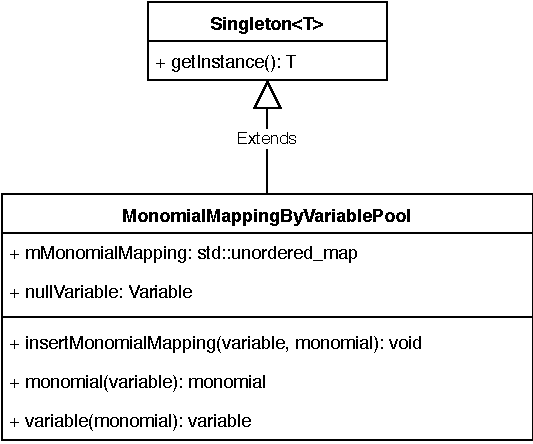
\includegraphics[width=0.6\linewidth]{./figures/MonomialMappingByVariablePool.pdf}
  \caption{Class diagram of \textit{mMonomialMapping}}
  \label{fig:class_diagram_of_mMonomialMapping}
\end{figure}

\noindent From the Figure \ref{fig:class_diagram_of_mMonomialMapping}, we can see there is an internal map \textit{mMonomialMapping} where we keep the Z-variables and multiplication terms.
We also declared a variable called \textit{nullVariable} which we used to represent a null variable.
The function \textit{insertMonomialMapping} takes a Z-variable and corresponding multiplication term as monomial and then insert into the internal map.
The function \textit{monomial} takes a Z-variable and searches it in the \textit{mMonomialMapping}.
If it finds the Z-variable, then returns the corresponding multiplication term as monomial.
Otherwise, it returns null pointer.
Similarly, the function \textit{variable} takes a multiplication term as monomial and searches it in the \textit{mMonomialMapping}.
If it finds the monomial, then returns the Z-variable.
Otherwise, it returns the \textit{nullVariable}.

%/////////////////////////////////////////////////
%/
\subsubsection{Generation of Axiom Formulas}
%/
%/////////////////////////////////////////////////
\label{subsubsec:Generation_of_Axiom_Formulas}
\textit{AxiomFactory} is a class that creates formulas for different axiom types.
As it creates formulas, we name it as \textit{AxiomFactory}.
We already know that there are five types of axioms in our work: zero axiom, monotonicity axiom, tangent plane axiom, congruence axiom and ICP axiom.
We have defined data type for each type of axiom in the enum class \textit{AxiomType} as follows:
\begin{table}[!ht]
\label{table:axiomType}
\centering
\begin{tabular}{|c|c|}
\hline
Axiom Type    & Data Type                                \\ \hline
zero          & \textit{ZERO}           \\ \hline
monotonicity  & \textit{MONOTONICITY}   \\ \hline
tangent plane & \textit{TANGENT\_PLANE} \\ \hline
congruence    & \textit{CONGRUENCE}     \\ \hline
ICP           & \textit{ICP}            \\ \hline
\end{tabular}
\end{table}

\noindent Figure \ref{fig:class_diagram_of_AxiomFactory} shows the class diagram of \textit{AxiomFactory}.
The class \textit{AxiomFactory} has a function \textit{createFormula} that creates axiom formulas depending on the parameter \textit{AxiomType}.
The function has another parameter of \textit{Model} type that is a model \textit{linearizedModel} containing the satisfying assignments for the elements of the map \textit{mMonomialMapping}.
We have mentioned it earlier in the section \ref{subsec:Refinement_Process} that the linearized model maybe incomplete for some multiplication terms which are stored in the map \textit{mMonomialMapping} against Z-variables and then we guess the values for the variables containing in those multiplication terms.
Therefore, we combine the linearized model \textit{mModel}, estimated assignments \textit{estimatedModel} for input NRA formula and guessed values for rest of the variables containing in the multiplication terms into the \textit{linearizedModel} and then it is passed to the function \textit{createFormula}.\newline

\noindent We create two Data Transfer Objects called \textit{VariableCapsule} and \textit{RationalCapsule}.
\textit{VariableCapsule} and \textit{RationalCapsule} encapsulate three \textit{Variable} objects and \textit{Rational} objects, respectively.
We introduce these data transfer objects to avoid long parameter list which is a type of code smell.\newline

\noindent We have defined different functions to generate formulas for different axiom types in \textit{AxiomFactory}.
We use SMT-RAT APIs to create the formulas in these functions.
If \textit{AxiomType} is \textit{ZERO} or \textit{TANGENT\_PLANE} or \textit{ICP}, we extract variables from each map element and the extracted variables will be encapsulated in \textit{VariableCapsule}.
Afterwards, we use this \textit{VariableCapsule} to generate formulas for the passed \textit{AxiomType}.
Remember that the list of different types of axioms are shown in Figure \ref{fig:List_Of_Axioms_For_Refining_Multiplication}.
When the \textit{AxiomType} is \textit{ZERO}, we only pass \textit{VariableCapsule} to create axiom formulas because we do not need assignments of the variables encapsulated in the \textit{VariableCapsule}.
Otherwise, for \textit{AxiomType} \textit{TANGENT\_PLANE} or \textit{ICP}, we pass both \textit{VariableCapsule} and \textit{RationalCapsule} to create axiom formulas.\newline

\begin{figure}[ht!]
  \centering
  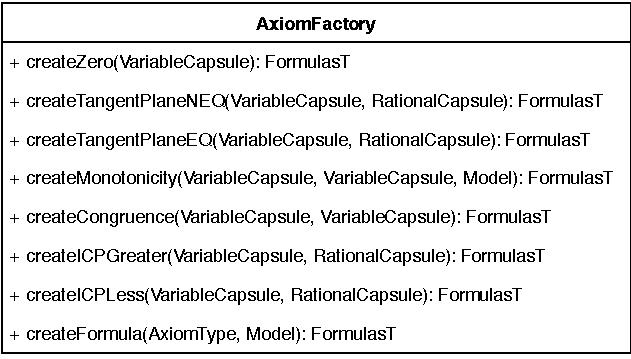
\includegraphics[width=0.6\linewidth]{./figures/AxiomFactoryClassDiagram.pdf}
  \caption{Class diagram of \textit{AxiomFactory}}
  \label{fig:class_diagram_of_AxiomFactory}
\end{figure}

\noindent If \textit{AxiomType} is \textit{MONOTONICITY} or \textit{CONGRUENCE} then similarly, we iterate over the map, but for each iteration, we iterate over the map again by a nested loop.
So, we have one outer and one inner loop.
Then, we have extracted variables to be encapsulated in \textit{VariableCapsule} objects for outer and inner loop.
Here first and second parameter of the functions \textit{createMonotonicity} and \textit{createCongruence} represents the  corresponding \textit{VariableCapsule} objects as outer and inner loop, respectively.
The function \textit{createMonotonicity} also has a third parameter of \textit{Model} type.
The implementation of \textit{createMonotonicity(VariableCapsule, VariableCapsule, Model)} is different from other formula creator functions and we will explain the implementation details in the next section.

%/////////////////////////////////////////////////
%/
\subsubsection{Generation of Formulas for Monotonicity}
%/
%/////////////////////////////////////////////////
\label{subsubsec:Generation_of_Formulas_ for_Monotonicity}
From Figure \ref{fig:List_Of_Axioms_For_Refining_Multiplication}, we can see that we have to generate axiom formulas for Monotonicity axiom with the absolute value of the variables i.e., $abs(x_{1}), abs(y_{1}), abs(z_{1})$ and so on, for each multiplication term.
There is no built-in function in SMT-RAT to create a formula with absolute value.
To solve this problem, first we create a equivalent formula for each absolute value of the variable ($x$) by introducing a new auxiliary variable ($aux\_x$) for $x$ as follows:
$$abs(x):= (x \geq 0 \to aux\_x = x) \quad \wedge \quad (x < 0 \to aux\_x = -x)$$
Then as shown in Figure \ref{fig:Equivalent_formula_for_a_constraint_with_absolute_value_of_variable}, we create equivalent formulas for each constraint i.e., $abs(x_{1}) \leq abs(x_{2})$, $abs(y_{1}) \leq abs(y_{2})$, $abs(z_{1}) \leq abs(z_{2})$ and so on, of the original Monotonicity axiom formulas (Figure \ref{fig:List_Of_Axioms_For_Refining_Multiplication}).
Note that in Figure \ref{fig:Equivalent_formula_for_a_constraint_with_absolute_value_of_variable}, the relation between two auxiliary variables depends on the relation between the absolute value of two variables of the constraint.
Finally, connect the equivalent formulas according to their connecting logical operators.\newline

\begin{table}[!ht]
\centering
\begin{tabular}{clc}
$abs(x_{1}) \leq abs(x_{2})$ := & $x_{1} \geq 0 \to aux\_x_{1} = x_{1}$  & $\wedge$  \\ 
  & $x_{1} < 0 \to aux\_x_{1} = -x_{1}$  & $\wedge$  \\ 
  & $x_{2} \geq 0 \to aux\_x_{2} = x_{2}$  & $\wedge$  \\ 
  & $x_{2} < 0 \to aux\_x_{2} = -x_{2}$  & $\wedge$  \\ 
  & $aux\_x_{1} \leq aux\_x_{2}$ &  \\ 
\end{tabular}
\end{table}
\begin{figure}[ht!]
\caption{Equivalent formula for a constraint with absolute value of variables}
\label{fig:Equivalent_formula_for_a_constraint_with_absolute_value_of_variable}
\end{figure}

\noindent In the Section \ref{subsec:Refinement_Process}, we see that how we find the unsatisfied axiom formulas to be added to the linearized formula.
The axiom formulas are called unsatisfied axiom formulas if they are not satisfied by linearized model.
But for \textit{AxiomType} \textit{MONOTONICITY} we cannot find the unsatisfied formulas until linearized model has the assignments for auxiliary variables.
That is why, we thought to create such a model which contains assignment for auxiliary variables  at the begining .
For this, we had to guess a value for each auxiliary variable.
We wanted to try two different values for each auxiliary variable (i.e., $aux\_x_{1} = x_{1}$ or $aux\_x_{1} = -x_{1}$ and $aux\_x_{2} = x_{2}$ or $aux\_x_{2} = -x_{2}$) containing in a constraint to check if the considered values validiate the equivalent formula of this constraint.
If we find such a value then we will assign this as a value to the auxiliary variable.
Otherwise, we can choose any of two different values.
So, for each constraint we have to try out four different combinations of values for the two auxiliary variables.
This solution can make our refinement process more costly and the performance may decrease a lot.
That is why, we do not pick this solution instead think about other optimized solution.\newline

\noindent We create a model \textit{absoluteValuedModel} which contains the absolute value of variables of the model \textit{linearizedModel}.
This \textit{absoluteValuedModel} is passed as the third parameter of the function \textit{createMonotonicity} which was mentioned in the previous section.
The function \textit{createMonotonicity} creates Monotonicity axiom formulas as shown in Figure \ref{fig:List_Of_Axioms_For_Refining_Multiplication} for a pair of multiplication terms and checks if these are unsatisfied by \textit{absoluteValuedModel}.
If unsatisfied formulas are found then their equivalent formulas are generated and accumulated into the \textit{List} \textit{monotonicityFormulas}.
Once all unsatisfied formulas are collected for that pair of multiplication terms, the function \textit{createMonotonicity} returns \textit{monotonicityFormulas} to its caller method.
%/////////////////////////////////////////////////
%/
\subsubsection{Module Settings}
%/
%/////////////////////////////////////////////////
\label{subsubsec:Module_Settings}
\begin{sloppypar}
We apply each possible combination of three heuristics and seven sequences of axiom types in the refinement process to find less costly pair of heuristic and sequence.
We need to declare them somewhere so that we can choose any combination easily.
SMT-RAT provides \textit{Settings} API by which we can declare various settings and afterwords we have to set the required settings in the strategy as module parameter.
At run-time, we can read the settings from the module and perform the selected settings specific operation.
So, we have to declare 21 different settings namely \textit{NRAILSettings$1$}, \textit{NRAILSettings$2$}, $\dots$, \textit{NRAILSettings$21$}.\newline

\noindent Now we will explain how we declare our different settings for \textit{NRARefinementSolver}.
Each settings must point to a heuristic and a sequence of axiom types.
We declare an enum class \textit{UNSATFormulaSelectionStrategy} to represent the heuristics.
This class has three enum types for \hyperref[item:heuristics]{three heuristics}: \textit{FIRST} for heuristic $1$, \textit{ALL} for heuristic $2$ and \textit{RANDOM} for heuristic $3$.
Each settings has one of this defined enum types.
Then we declare a sequence of axiom types in an array by putting the \hyperref[table:axiomType]{enum types of enum class \textit{AxiomType}} sequentially.
This array contains one of the \hyperref[item:sequences]{sequences (Sequence $1$, $\dots$, Sequence $7$)}.
So, the refinement process is performed over the axiom types in the same sequence as decelerated in the selected settings and collects unsatisfied formulas according to defined heuristic in that settings.
We have considered \textit{NRAILSettings$1$} as our default settings \ref{lst:default_settings}.\newline
\end{sloppypar}

\begin{figure}[!ht]
\begin{lstlisting}[language=C++,label=lst:default_settings, caption={Default settings}]
struct NRAILSettings1
{
 moduleName = "NRAILModule<NRAILSettings1>";

 UNSATFormulaSelectionStrategy 
 formulaSelectionStrategy = UNSATFormulaSelectionStrategy::ALL;

 AxiomFactory::AxiomType
 axiomType[5] = {AxiomFactory::AxiomType::ZERO,
	         AxiomFactory::AxiomType::TANGENT_PLANE,
		 AxiomFactory::AxiomType::ICP,
		 AxiomFactory::AxiomType::CONGRUENCE,
		 AxiomFactory::AxiomType::MONOTONICITY};
};
\end{lstlisting}
\end{figure}

\noindent As we have 21 diffrent settings, we have also created 21 different strategies namely \textit{NRARefinementSolver$1$}, \textit{NRARefinementSolver$2$}, $\dots$, \textit{NRARefinementSolver$21$} with \textit{NRAILSettings$1$}, \textit{NRAILSettings$2$}, $\dots$, \textit{NRAILSettings$21$}, respectively.
Each of them are copies of \textit{NRARefinementSolver} shown in Figure \ref{fig:overview_architecture_SMT-RAT} but with corresponding settings as module parameter.
The strategy \textit{NRARefinementSolver} has the default settings.\newline